% Note: To remove the "DRAFT VERSION" warnings, replace the following line with:
% \documentclass[final]{cubedoc}
\documentclass[final]{cubedoc}

\title{A short thermal properties journey for the PCB/package level} %% Assignment Title
\docid{AcubeSAT-THE-BH-032}

\author{Theodoros Katzalis}

\changelog{15/04/2020}{0.1}{DRAFT}{Initial revision}
\changelog{15/04/2020}{0.2}{INTERNALLY RELEASED}{First release}
\changelog{18/08/2020}{0.3}{INTERNALLY RELEASED}{Updated:
	\begin{itemize}
		\item Fix typos and rephrasing.
		\item Table \ref{tab:plate}: Heat Capacity of Tin changed from 0.226 to 226.
	\end{itemize}
	\bigskip
	
	Added:
	\begin{itemize}
		\item Tables \ref{fig:tab_1}, \ref{fig:tab_2}
		, \ref{fig:tab_3}, \ref{fig:tab_4}.
		\item Footnote for .bxl extension.
		\item Image sources and archive websites.
	\end{itemize}
}

\usepackage{tablefootnote}
\usepackage{longtable}
\usepackage{multirow}
\usepackage{supertabular}
\usepackage{adjustbox}
%\usepackage{indentfirst}
\usepackage{subcaption}
\usepackage{graphicx}
\usepackage{hyperref}
\usepackage{cleveref}


%\hypersetup{
%    colorlinks=true,
%    urlcolor=blue,
%    linkcolor=black,
%    citecolor=black
%}


\begin{document}
	
	\section{Introduction}
	
	This is a \textbf{summary} report for the research about thermal properties of the materials used for AcubeSAT's PCBs. A bunch of resources, documentation and issues are listed because during the process some conflicts and uncertainties emerged. I should mention that thermal analysis is very demanding and complex topic, so the documentation of the resources and thinking-paths are valuable tools to spot the possible wrong assumptions and \textbf{fallacies}. \textbf{The until now estimating values for this research can be found in \href{https://drive.google.com/open?id=1gGPhBZe94Yt7D8FDdGNza4ZnG0pRfhT0xG7Z2tBdK7o}{this} spreadsheet}.
	
	\section{Electronic packaging}
	
	There are many reference points that the electrical components can be grouped. The most common one is based on how they interconnect with the PCB. If holes should be used, then we are using the through hole technology (\textbf{THT}) and if the device is mounted, then we are using the surface mount technology (\textbf{SMT}). The devices that are using the last one, as an interconnection method, are called SMDs and they can be divided to many categories too. For now, we will divide them to the \textbf{leaded} and the \textbf{leadless}. In the first belong the packages that their leads extend beyond the package and in the second when they don't. We are going to focus in the SMDs because if not everything, almost all the components that are going to be used in the AcubeSAT's boards, except the PC104 connectors, will use the SMT. 
	
	Before diving into what is hidden under the hood of the black boxes that we are looking in the PCB, we need first to demystify the terminology. \textbf{Packaging} is an abstract word and is used a lot in the electronics but it has several meanings and "thought layers". There are the chip packaging, the PCB packaging and the systems packaging where a lot of PCBs are interconnected with each other. In a different way, packaging can be referred to \textbf{integrated circuit} and \textbf{electronic}. Electronic packaging has to do with everything about the interconnection of the die with the external circuitry of a PCB. The integrated circuit packaging is actually the last step of the electronic one. It is referred to the encapsulation process, the protection of the IC from the rest of the environment.
	
	But lets stay more in the electronic packaging definition. There are four main levels:
	
	\begin{enumerate}
		\item \textbf{Semiconductor} (or die, chip, IC) level. The wafer is separated into chips and one of them is inside of the package. The die, most of the times, is Si based, but GaAs can be used for high speed applications. In the die level, metalization (Al, Cu, Ag) takes place for oxidation protection.
		\item \textbf{Chip in a carrier}. This is where all the bonding takes place. The die is attached to a leadframe or a substrate  and the wire bonds serve the role of interfacing the integrated circuit with the outer leads (these terms will be explained soon). For the die attachment we have conductive or non conductive adhesive (but always thermal conductive) . If there is an exposed pad for example and electrical connection is desired, then the first one is used\footnote{Most of the times the exposed pad will be grounded but you need to be sure checking the datasheet otherwise problems may occur.}. 
		\item \textbf{PCB level}. The chip is mounted on the board either with leads or no leads. Then the leads via copper tracks are connected with other components.
		\item \textbf{System level}, PCB to PCB interconnect. This is where multiple PCBs are connected all together for a large application.
	\end{enumerate}
	
	In order to understand a little bit more all of these new/fuzzy terms like die, leadframe, substrate, wirebonds (bonding-wires), we will give an example of a package based on the through-hole technology. Thus let's take a look of a very well-known package that showed among the first ones in the job market. This is the dual line package (\textbf{DIP}). As we can see, the leadframe is the structure that houses the chip and interfaces the integrated circuit with the leads. The interface that change the pitch from the die to the outer leads is called \textbf{interposer}. Sometimes leadframe and interposer are used interchangeably. The material used in the leadframe is copper or copper alloys and it is usually plated with tin or gold over nickel for oxidation-protection and to ensure wirebondability and solderability for the assembly process. The die is attached to the leadframe pad using an organic compound (die attachment), epoxy resin with metal fillers (e.g. silver). Finally, for the encapsulation, the most used and cost-effective solution is the plastic package. It is epoxy resin with ceramic fillers like fused silica or alumina. It should be noted that \textbf{mold compounds} are called the materials used in the encapsulation process. 
	
	\begin{figure}[h!]
		\centering
		\begin{subfigure}{.5\textwidth}
			\centering
			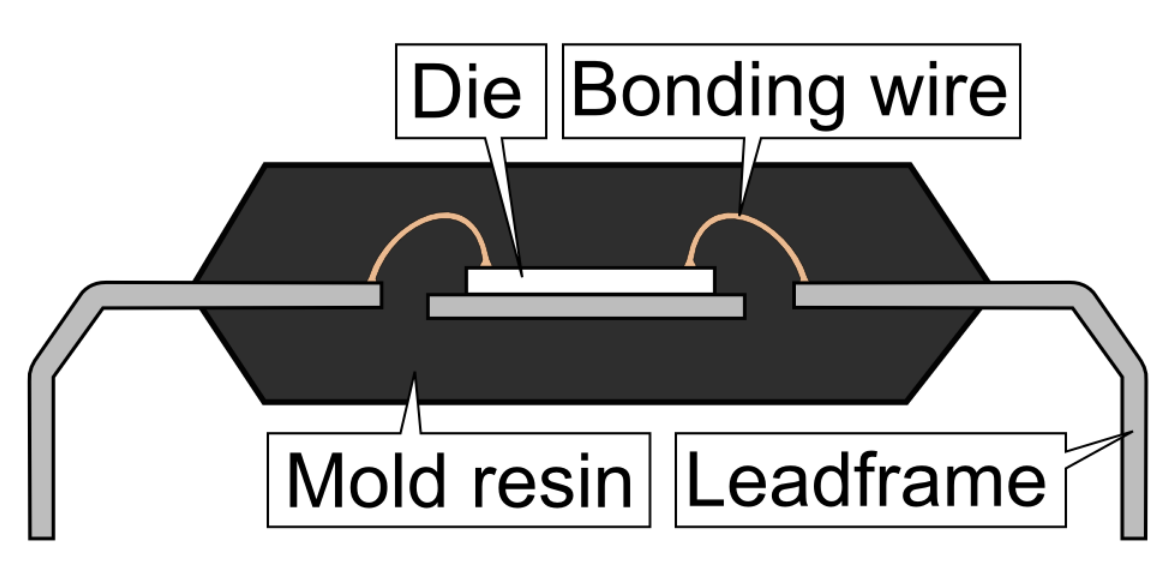
\includegraphics[width=0.7\linewidth]{docs/pdip.png}
			\caption{DIP cross section view \small{(\href{https://web.archive.org/web/20200818152711/https://commons.wikimedia.org/w/index.php?title=File:DIP_package_sideview.PNG&oldid=131332920}{image source})}}
			\label{fig:sub1}
		\end{subfigure}%
		\begin{subfigure}{.5\textwidth}
			\centering
			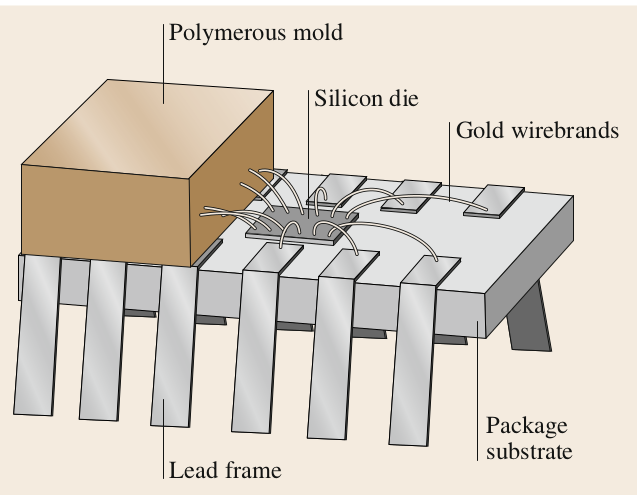
\includegraphics[keepaspectratio, width=0.7\linewidth, height=.4\textheight]{docs/dip_leadframe.png}
			\caption{DIP leadframe \small{(\href{https://web.archive.org/web/20200818152844/https://link.springer.com/chapter/10.1007/978-3-319-48933-9_530}{image source})}}
			\label{fig:sub2}
		\end{subfigure}
		\caption{}
		\label{fig:test}
	\end{figure}
	
	The DIP package that we have mentioned belongs to the plastic leadframe-based packages. That implies that the IC packaging can be, for once more, categorized in terms of material packaging to the \textbf{plastic and ceramic} ones and in terms of housing/supporting the die to the \textbf{leadframe and the substrate}.
	
	For the difference between the ceramic and the plastic we are going to use the Cer-DIP as an example. Yes you guess right, it is a DIP but with ceramic materials for the packaging. So, a typical ceramic package has a ceramic base/leadframe that is embedded to glass and a lid. The ceramic material that is used most often is the Aluminum oxide (alumina) and for the lid, metal or ceramic ones. The benefits of ceramic packaging is the hermetic feature, the increased reliability and the greater thermal conductivity (one order of magnitude more) than plastic polymeric epoxy resin based packages. The main drawback is the cost and thus it is avoided for mass production. 
	
	\begin{figure}[h!]
		\centering
		\begin{subfigure}{.5\textwidth}
			\centering
			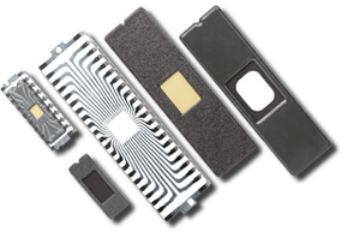
\includegraphics[height=0.2\textheight, width=\textwidth, keepaspectratio]{docs/cer_dip_real.png}
			\caption{Three main parts of a CER-DIP: base,\\ 
				leadframe, lid  \small{(\href{https://web.archive.org/web/20200818153119/https://www.spectrum-semi.com/cerdip}{image source}})}
			\label{fig:sub1}
		\end{subfigure}%
		\begin{subfigure}{.5\textwidth}
			\centering
			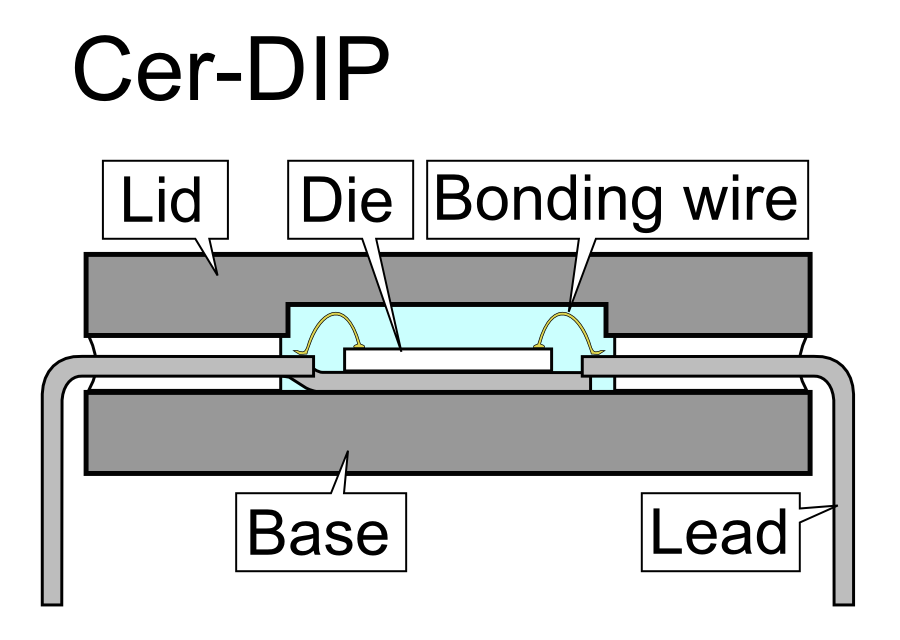
\includegraphics[height=0.2\textheight, width=\textwidth, keepaspectratio]{docs/cdip.PNG}
			\caption{Cross section view of a ceramic package \small{(\href{https://web.archive.org/web/20200818153102/https://commons.wikimedia.org/wiki/File:Cer-DIP_package_sideview.PNG}{image source})}}
			\label{fig:sub2}
		\end{subfigure}
		\caption{}
		\label{fig:test}
	\end{figure}
	
	Before proceeding further, for one more time we will make another division and we will describe the leadframe-based and the substrate packages.
	For the leadframe style we have mentioned the DIP, but what about the substrate-style? So to understand this, we will make a huge jump and we will move to a more advanced packaging method, to the family of grid array and more specific to the Land Grid Array (\textbf{LGA}). In this category is included the component RFFM6406 UHF TX-RX of the communication subsystem so it is sure worth describing, or I should say scratching the surface of this type. A general cross view of a LGA is like this (Figure \ref{fig:sub2}). The die is now glued, instead of a leadframe, to a substrate that is actually a laminate that is like a PCB! So we have a "PCB inside a PCB". It may have a lot of copper and dielectric layers along with soldermask to the top. The die is attached to the top layer. Then the wirebonds are attached to some exposed copper areas of the top layer and with vias the integrated circuit is now connected to the exposed pads in the bottom surface that serve the interface of the die with the rest of the circuit. This type of packages are used in demanding applications for high speed signals that its thermal and electrical performance is crucial and for populated areas with no room to breathe due to the small size but the increased functionality! 
	
	
	\begin{figure}[h!]
		\centering
		\begin{subfigure}{.3\textwidth}
			\centering
			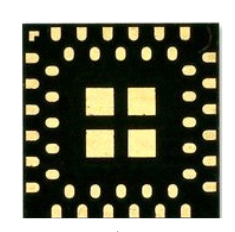
\includegraphics[keepaspectratio, height=.4\textheight, width=\textwidth]{docs/lga.png}
			\caption{Bottom side \small{(\href{https://web.archive.org/web/20200818134018/https://www.nxp.com/docs/en/application-note/AN2265.pdf}{image source})}}
			\label{fig:sub1}
		\end{subfigure}%
		\begin{subfigure}{.6\textwidth}
			\centering
			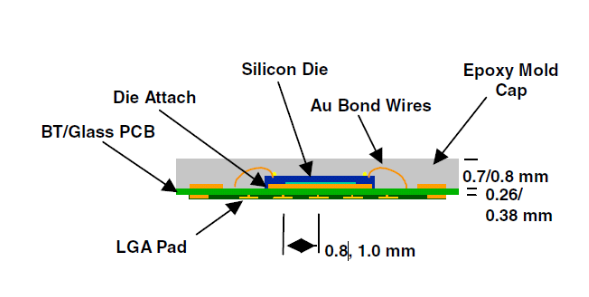
\includegraphics[keepaspectratio, width=\textwidth, height=.6\textheight]{docs/lga_cross.png}
			\caption{Cross section view \small{(\href{https://web.archive.org/web/20200818134018/https://www.nxp.com/docs/en/application-note/AN2265.pdf}{image source})}}
			\label{fig:sub2}
		\end{subfigure}
		\caption{LGA}
		\label{fig:test}
	\end{figure}
	
	
	Now that we have an \textbf{overview} of the packaging and the terminology, we are going to examine the packages of the components of the AcubeSAT's board that we assume as critical from a thermal's point of view. The list of these can be found in the aforementioned spreadsheet\footnote{This report may be outdated in the long run if more packages are going to be added}. It should be noted that the following analysis of the IC packages isn't complete and it isn't oriented for a detailed 3D IC simulation. The goal is to find out if we need to create eventually these kind of detailed models based to the materials and their thermal properties that will be listed in the continue of this report. So if eventually a more detailed approach  is necessary, thorough investigation should be made for the standardized dimensions of the internal structure of each package. 
	
	It should be noted that the \textbf{material declaration}, the document that lists all the materials used in packaging, isn't provided for all of them. To be more specific this particular type of doc is successfully indexed from manufacturers such as ST Microelectronics, Texas Instruments (TI) and Analog Devices that generally have great documentation and support. For the rest, by the code-name\footnote{The IC package naming convention is a function of the physical dimensions, pins, pitch and the overall anatomy of the package. Most of them are standardized but vendors may use different names} of the package (e.g. QFP, SOIC), we can safely think abstractly for the anatomy and the materials used. This is not accurate, but it bares the risk for the scope of this report. In other words, if the package is a well known and among the standardized ones, there are many chances that will be identical with other references that using the same package (of course some details may be different). For these with the missing material declaration, if we are finally going to follow the detailed approach, we need, except the standardized dimensions, to contact the vendor and request more information (it is worth mentioning that this kind of contact may be unsuccessful, so a more "delicate" approach would be more suitable). 
	
	
	\subsection{LQFP}
	
	
	LQFP stands for Low profile Quad Flat Package, it has 144 pins and belongs to the very well-know QFP series. There are slight variations for the physical dimensions of the components associated with this code-name, but the AcubeSAT's components with this tag are all the same. These are the \textbf{OBDH, SU and ADCS MCU}.
	
	First, from the material declaration (see the complete document \href{https://web.archive.org/web/20200818131830/https://www.st.com/content/ccc/resource/quality_and_reliability/quality_certificate/material_declaration/group3/be/7d/54/2a/11/68/4e/ad/DM00442253/files/P41A_470XXXY_signed.pdf/jcr:content/translations/en.P41A_470XXXY_signed.pdf}{here}) we can validate that it is a plastic leadframe-based package. But let's make a summary for the listed-materials.
	
	%Oh god, I need to create a table??
	
	\begin{table}[h!]
		\centering
		\begin{tabular}{ |c|c|c| }
			\hline
			\multirow{1} {*} {\textbf{Parts}} & \textbf{Material} & \textbf{Mass} \\  
			\hline
			\multirow{8} {*} {Die}  & Silicon & 24.184 \\ \cline{2-3} & Aluminum & 0.045 \\ \cline{2-3} & Copper & 0.397 \\ \cline{2-3} & Cobalt & 0.001 \\ \cline{2-3} & Tantalum & 0.129 \\ \cline{2-3} & Titanium & 0.005 \\ \cline{2-3} & Tungsten & 0.003 \\ \cline{2-3} & Silicon Nitride & 0.101 \\ \cline{2-3} & Silicon Oxide & 0.257  \\
			\hline
			\multirow{4} {*} {Leadframe base}  & Copper & 233.880 \\ \cline{2-3} & Iron & 5.760 \\ \cline{2-3} & Zinc & 0.288 \\ \cline{2-3} & Metallic Phosphorous & 0.072 \\ 
			\hline
			\multirow{3} {*} {Leadframe plating}  & Nickel & 9.021 \\ \cline{2-3} & Palladium & 0.140 \\ \cline{2-3} & Gold & 0.140 \\ 
			\hline
			\multirow{7} {*} {Die attachment}  & Copper & 2.170 \\ \cline{2-3} & Iron & 0.155 \\ \cline{2-3} & Silica fused & 0.310 \\ \cline{2-3} & Metallic Phosphorous & 0.016 \\ \cline{2-3} & Diluent & 0.155 \\ \cline{2-3} & Allyl Compound & 0.155 \\ \cline{2-3} & Hardener & 0.140 \\
			\hline
			\multirow{4} {*} {Bonding wires}  & Gold & 2.376 \\ \cline{2-3} & Palladium & 0.024 \\ \cline{2-3} & Silver & 0.000 \\ \cline{2-3} & Copper & 0.000 \\
			\hline
			\multirow{6} {*} {Encapsulation}  & Epoxy resin A & 20.706 \\ \cline{2-3} & Epoxy resin B & 41.412 \\ \cline{2-3} & Silica Amorphous A & 811.789 \\ \cline{2-3} & Silica Amorphous B & 88.001 \\ \cline{2-3} & Carbon Black & 5.177 \\ \cline{2-3} & Phenol resin & 67.295 \\
			\hline
			\multirow{3} {*} {Finishing}  & Nickel & 0.679 \\ \cline{2-3} & Palladium & 0.011 \\ \cline{2-3} & Gold & 0.011 \\ 
			\hline
		\end{tabular}
		\caption{Material declatation OBC MCU}
		\label{tab:matdoc}
	\end{table}
	
	
	As we can see in the table \ref{tab:matdoc}, in the die level, the base material is the Silicon and all the other metals are used for the so called metallization that serves the role of oxidation protection for the chip. The die attachment is a typical epoxy resin with silver as filler metal and for the leadframe we have a copper alloy that it is pre-plated with nickel over gold.
	
	
	\begin{figure}[h!]
		\centering
		\begin{subfigure}{.5\textwidth}
			\centering
			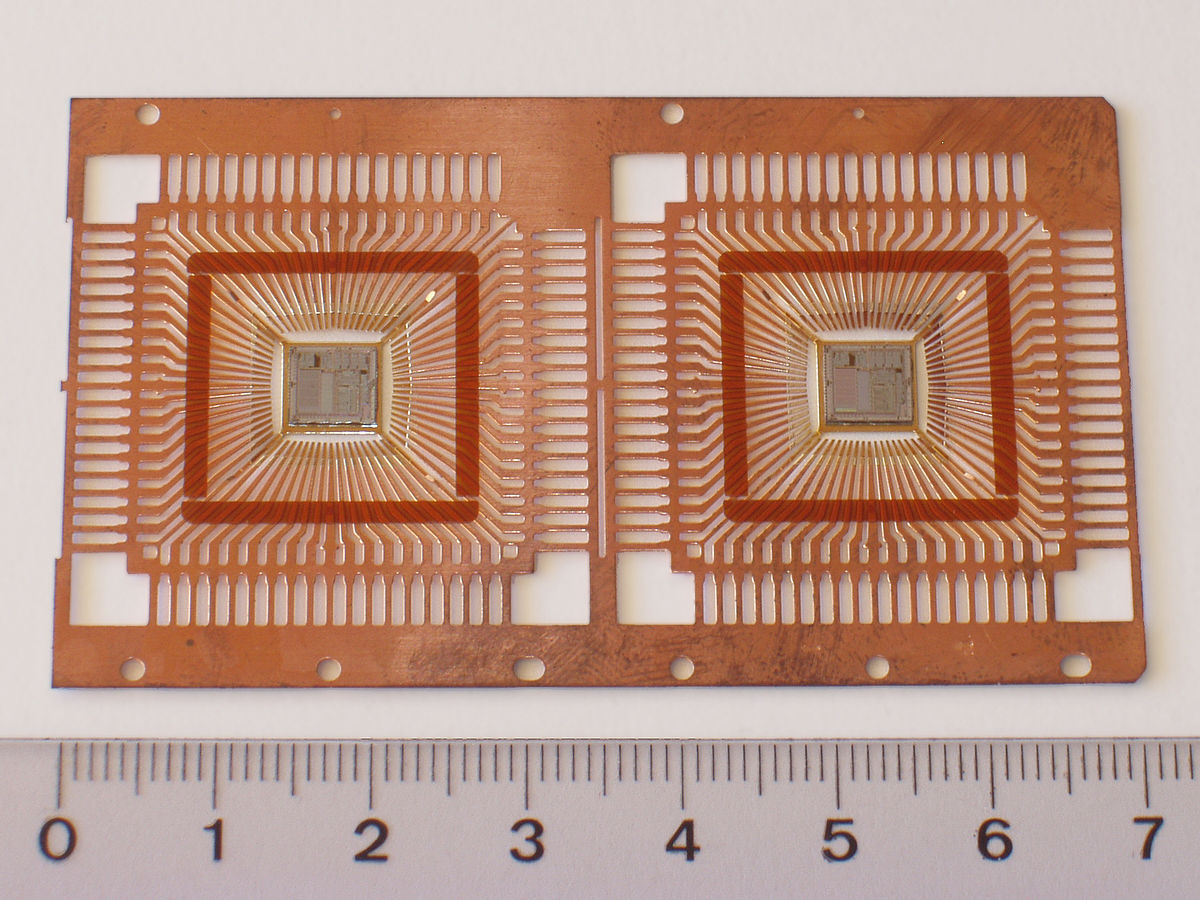
\includegraphics[keepaspectratio, width=0.7\linewidth]{docs/leadframe_qfp.jpg}
			\caption{Two QFP leadframes \small{(\href{https://web.archive.org/web/20200818153249/https://commons.wikimedia.org/wiki/File:TQFP_Leadframe.jpg}{image source})}}
			\label{fig:sub1}
		\end{subfigure}%
		\begin{subfigure}{.5\textwidth}
			\centering
			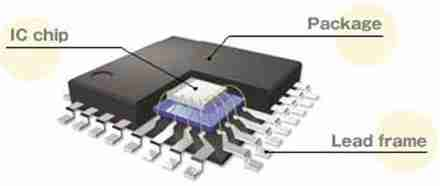
\includegraphics[keepaspectratio, width=\linewidth, height=.6\textheight]{docs/qfp_anatomy.jpg}
			\caption{QFP package anatomy \small{\href{https://web.archive.org/web/20200818153744/http://resource.renesas.com/lib/eng/fab/index.html}{image source}}}
			\label{fig:sub2}
		\end{subfigure}
		\caption{}
		\label{fig:test}
	\end{figure}
	
	\subsubsection{Thermal properties}
	
	
	About the thermal properties, an all in one solution for the requested ones (thermal conductivity, heat capacity, absorptivity, emissivity) couldn't be indexed. Instead a lot of references have been found scattered around the web. Of course, there are some deviations/conflicts among these references. For now, we are going to list the materials and its properties of the most used ones in the IC packaging. We are going to assume the die as only silicon, the leadframe as a \textbf{copper alloy} (Cu-Fe) plated with gold over nickel, the wirebonds as gold and the encapsulation as an abstract \textbf{epoxy mold compound} (EMC)\footnote{For thermal conductivity of various EMC with different fillers see Table I of \cite{Cheng2018StudyOT}}. For more materials, some tables have been added to the end of this report (\cref{list_tables}) along with their references. Also there is the \cref{Databases} with databases for thermal properties for further investigation. About how to approach the thermal properties of the materials, some comments have been added to the Lessons learned (\cref{lessons_learned}).
	
	\begin{table}[h!]
		\centering
		%\tablehead{\hline}
		%\tabletail{\hline}
		%\tablecaption{Summary of the material declaration of LQFP package}
		\resizebox{\textwidth}{!}{\begin{tabular}{ |c|c|c|c|c| }
				\hline
				\multirow{1} {*} {\textbf{Substance}} & \textbf{Density ($kg/m^3)$} & \textbf{Thermal Conductivity ($W/m*K)$} & \textbf{Heat Capacity ($J/kg*C)$} & \textbf{References respectively} \\
				\hline
				\multirow{1} {*} {Silicon}  & 2330 &  150 & 714 & Figure \ref{fig:springer_properties} \\ 
				\hline
				\multirow{1} {*} {Cu-Fe}  & - & 260 & - & Figure \ref{fig:copper_alloys} \\
				\hline
				\multirow{1} {*} {Epoxy mold compound}  & 1790-1850 & 0.9-2 & 800 & \href{https://web.archive.org/web/20200818132142/https://www.intel.com/content/dam/www/public/us/en/documents/packaging-databooks/packaging-chapter-05-databook.pdf}{link}, \href{https://web.archive.org/web/20200818132243/https://www.ti.com/lit/an/spra953c/spra953c.pdf}{link}, \href{https://web.archive.org/web/20200818132309/https://www.caplinq.com/blog/heat-capacity-of-epoxy-molding-compound_102/}{link} \\
				\hline
				\multirow{1} {*} {Plating Ni/Au/Pd}  & - & - & - & - \\
				\hline
		\end{tabular}}
		\caption{Material Bulk properties of QFP}
		\label{tab:my_label}
	\end{table}
	
	For the thermo-optical properties, in general we are interested for the outer surfaces, like the encapsulation of package (epoxy mold compound or ceramic) and the leads (copper alloy plated with Nickel/Gold/Palladium aka Copper electroplated)
	\begin{table}[h!]
		\centering
		%\tablehead{\hline}
		%\tabletail{\hline}
		%\tablecaption{Summary of the material declaration of LQFP package}
		\begin{tabular}{ |c|c|c|c| }
			\hline
			\multirow{1} {*} {\textbf{Substance}} & \textbf{Emissivity} & \textbf{Absorptivity} & \textbf{References respectively}\\  
			\hline
			\multirow{1} {*} {Copper electroplated} & 0,03 & 0,47 & \cite[p.346]{chhabra2017crc} \\  
			\hline
			\multirow{1} {*} {Epoxy mold compound} & 0,9-0,95 & -  & \cite[p.9]{renesasmetric} \\  
			\hline
		\end{tabular}
		\caption{Thermo-optical properties}
		\label{tab:my_label}
	\end{table}
	
	
	Reference for an homogenous approach of the plating Nickel/Gold/Palladium is also missing, but thermal properties for each one of these metals are easily available. For accuracy and more information (such as thickness\footnote{ \href{https://web.archive.org/web/20200818132539/https://www.idt.com/us/en/support/knowledge-base/what-are-specifications-terminal-plating-plating-methods-and-plating-thickness-any-idt-part}{Reference} for plating thickness} for the plating materials) we may need to research more about the IC assembly.
	
	\begin{table}[h!]
		\centering
		%\tablehead{\hline}
		%\tabletail{\hline}
		%\tablecaption{Summary of the material declaration of LQFP package}
		\resizebox{\textwidth}{!}{\begin{tabular}{ |c|c|c|c|c| }
				\hline
				\multirow{1} {*} {\textbf{Substance}} & \textbf{Density ($kg/m^3)$} & \textbf{Thermal Conductivity ($W/m*K)$} & \textbf{Heat Capacity ($J/kg*C)$} & \textbf{References respectively} \\
				\hline
				\multirow{1} {*} {Nickel}  & 8908 &  92 & 440 & \cite{engtooldensity}, Figure \ref{fig:intel_conduct},  \cite{engtoolcapacity} \\ 
				\hline
				\multirow{1} {*} {Gold}  & 19320 & 297 & 130 & \cite{engtooldensity}, Figure \ref{fig:intel_conduct}, \cite{engtoolcapacity}\\
				\hline
				\multirow{1} {*} {Palladium} & 12160 & 71.8 & 240 & \cite{engtooldensity}, Figure \ref{fig:metal_table_2}, \cite{engtoolcapacity} \\
				\hline
				\multirow{1} {*} {Tin} & 5765 & 63.2 & 226 & \cite{azomtin}, \cite{azomtin}, \cite{engtoolcapacity}\\
				\hline
		\end{tabular}}
		\caption{Material Bulk properties of plating-metals}
		\label{tab:plate}
	\end{table}
	
	
	\subsubsection{Lead-PCB interconnection}
	
	
	Plating is a process involved not only in the PCB but in the IC fabrication too. The goal is to ensure solderability and additional protection from oxidation and other environmental concerns. In other words, plating serves the role to bond two un-solderable surfaces. In the PCB phase, the exposed copper (pads) is plated with electroless gold over nickel and tin. For the IC phase, the base metal of the terminals aka leads are plated either with matte tin (Sn) as a surface treatment (after the mold-process used for the encapsulation) or with  nickel/palladium/gold (Ni/Pd/Au) that is pre-plated in the leadframe. So far, the PCB and the IC have solderable surfaces and the only thing left for the bonding is the soldering by the assembly house using either solder paste or electrically conductive adhesive (ECA).  
	
	
	The "stack-up" is actually in simple terms: plated terminals (leads or pads. For this package we have leads) then the solder paste (or conductive adhesive) and then the plated exposed copper of the board. 
	
	
	\begin{figure}[h!]
		\centering
		\begin{subfigure}{.5\textwidth}
			\centering
			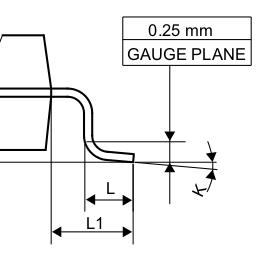
\includegraphics[width=0.7\linewidth]{docs/gullwing_leads.png}
			\caption{OBC MCU Mechanical drawing}
			\label{fig:sub1}
		\end{subfigure}%
		\begin{subfigure}{.5\textwidth}
			\centering
			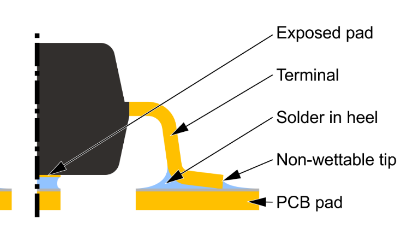
\includegraphics[keepaspectratio, width=1.3\linewidth, height=.4\textheight]{docs/gullwing_solder.png}
			\caption{A perfect soldering of the lead with PCB \small{(\href{https://web.archive.org/web/20200818154144/https://www.infineon.com/dgdl/Infineon-Board+Assembly+Recommendations-Gullwing-Package-v04_00-EN.pdf?fileId=5546d4626d82c047016d8c0320de42d0}{image source}})}
			\label{fig:sub2}
		\end{subfigure}
		\caption{}
		\label{fig:test}
	\end{figure}
	
	
	
	Now let's examine the dimensions of these gullwing\footnote{The J shaped leads are the so called gullwing leads} leads. The range of values for the depicted L parameter, according to the OBC MCU datasheet, is 0,45 - 0,750 mm and the typical value is 0,6 mm. As we can see from the figures, the exact contact area is a little bit unclear. The solder paste is applied to the whole surface of the PCB pad (this is valid from the .bxl files\footnote{.bxl file extension is a vendor standardized format that can be used via Ultralibrarian software to export data such as schematic symbols, footpritns, 3D models compatible for a wide range of CAD tools.} from ST Microelectronics in which there is metadata for the solder paste layer) and only the L part of the lead is attached to the solder. But all together are electrical and thermal conductive. So we can assume as contact area the PCB pad? In other words the contact area is the L * (width of the lead, that is typically 0.220 mm) or the soldered PCB pad (1.35 * 0.35 mm). It is worth mentioning also that leadframe based packages don't usually touch the surface of the PCB due to the \textbf{standoff} height. The value for this based on the mechanical drawing can range from 0.050 - 0.150.
	
	In order to determine the thickness of the solder paste we need to know the stencil design. A typical value will be 130um.
	
	
	\subsubsection{Soldering}
	
	
	For the bonding of two metal surfaces there are two main methods: 1) \textbf{electrical conductive adhesive} and 2) \textbf{solder paste} (solder with flux). 
	
	
	Conductive adhesive is a composite of thermosetting epoxy adhesive resin and conductive metal (or metal-coated) particles, such as silver, nickel, gold, copper and indium or tin oxides. On the other hand, the solder is a metal alloy and can be divided to the solder with lead (tin-lead, SnPb) and the lead-free. For the first, the most common is the 63Sn37Pb, but due to environmental and health concerns, lead usage is prohibited by regulations (RoHS, REACH) so manufacturers are tending to avoiding it. Tin (Sn) and tin-silver-copper (SnAgCu) belong to the lead-free group. In terms of thermal performance, thermal conductivity is higher in solders (60-65 W/mK) than adhesives (3-25 W/mK) \cite{leadvssolde}. 
	
	The assembly provider of the in-house AcubeSAT's PCBs is Prisma Electronics. It is unclear which of these two methods in the FM models will be used, so clarifications should be requested. Nevertheless if we know the type, then we can retrieve thermal data from these references \cite{solder, wiki:solderalloys, propemetalengedge}.
	
	
	\subsubsection{Closing}
	
	
	If you have stayed until the end of this package analysis you will realized that the die anatomy and what is inside of the black box is a little bit complex from a thermal's point of view because there is a variety of materials that can be used and many surfaces are touching each other with different physical (thickness, size) and thermal characteristics. For the rest of the packages we will not approach them with the same detail. We will make an overview and if more accurate thermal data is required for the packaging, further research should be made!
	
	
	\subsection{TSOP}
	
	
	
	Another package, that is included in the group of packages used in the AcubeSAT's boards, is the thin small outline package (TSOP). All the memory modules belong to this category (OBDH MRAM, ADCS SRAM, SU SRAM, SU NAND). This type of package has the leadframe-style and  the mechanical dimensions of the gullwing leads for OBDH, ADCS and SRAM are the same with the previous LQFP and for the SU NAND, the range is 0.4-0.6 with typical 0.5 mm. 
	
	For each one of the memory modules the material declaration is not included in the docs, so we don't know: 1) the terminal plating, 2) base material for the leads. Specifically for OBDH MRAM, from \href{https://www.everspin.com/supportdocs/MR0A16AYS35R?npath=}{a product change notification} about the molding compound used, we can see the code-name "\textbf{Sumitomo G631H}" that is the same in the material declaration of the ST's LQFP packages. So for the Everspin's MRAM we can safely assume that the encapsulation characteristics are the same with the LQFP. For the terminals plating we can assume again that the base material is copper or a copper alloy (or iron\footnote{The material declaration \cite{alliancematdoc} for another TSOP product by Alliance indicates leadframe is iron-based} based) with tin or nickel over gold plating. For clarification, we should contact the vendor.
	
	About the NAND memory module, according to the \href{https://drive.google.com/file/d/1wkUdeeUTbI0Y1cVbS6Vn8aBa2U0LKccN/view?usp=sharing}{user guide}, the leadframe is plated with the usual matte tin or Ni/Pd/Au and the thickness is specified, but it isn't clarified which one of these is used in our particular module. The thickness though is a valuable info (for the standardized world of electronics) and we can use it as a general reference for plating leadframe thickness too.
	\begin{itemize}
		\item Nickel 0.5 um to 1.2 um
		\item Gold 0.003 to 0.012 um
		\item Palladium 0.03 um to 0.11 um
	\end{itemize}
	
	
	
	\begin{figure}[h!]
		\centering
		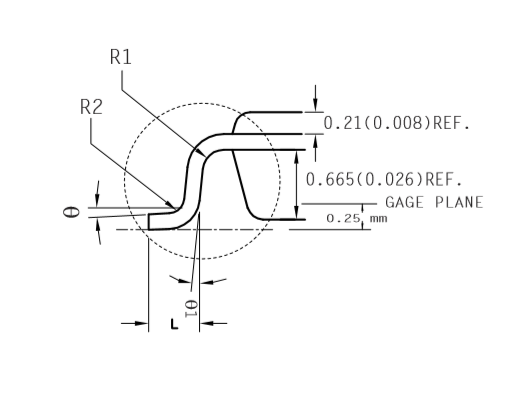
\includegraphics[height=0.3\textheight, width=\textwidth, keepaspectratio]{docs/gullwing_leads_TSOP.png}
		\caption{Gullwing leads for the TSOP2 package by MRAM technical note}
		\label{fig:my_label}
	\end{figure}
	
	\subsection{QFN}
	
	
	Quad Flat No-leads (QFN) package is used for the COMMS AT86RF215 UHF TX-RX. It belongs in the leadless family and includes an exposed thermal pad for heat dissipation (it is recommended to use vias). Usually the package is plastic and the leadframe copper but the material declaration is missing for this specific component. 
	
	It should be emphasized that although there are no leads, according to the datasheet the standoff height range is 0 - 0.05mm (typical 0.02mm).
	
	\begin{figure}[h!]
		\centering
		\begin{subfigure}{.5\textwidth}
			\centering
			\includegraphics[keepaspectratio, width=0.8\linewidth, height=.4\textheight]{docs/qfn_sideview.png}
			\caption{}
			\label{fig:sub1}
		\end{subfigure}%
		\begin{subfigure}{.5\textwidth}
			\centering
			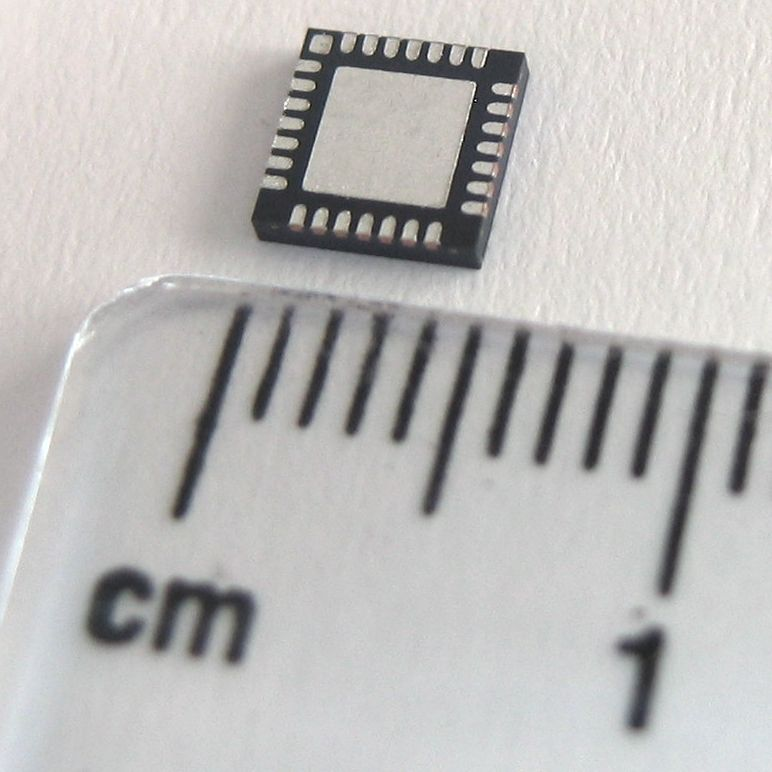
\includegraphics[keepaspectratio, width=0.5\linewidth, height=.3\textheight]{docs/qfn_real.jpg}
			\caption{}
			\label{fig:sub2}
		\end{subfigure}
		\caption{QFN \small{(\href{https://web.archive.org/web/20200818153946/https://en.wikipedia.org/wiki/Flat_no-leads_package}{image source})}}
		\label{fig:test}
	\end{figure}
	
	
	
	\subsection{SOIC}
	
	A Small Outline Integrated Circuit (SOIC) is the package of the EPS TPS54339EDDA. It has 8 pins with an exposed pad. The  \href{https://web.archive.org/web/20200818133800/https://www.ti.com/materialcontent/en/report?pcid=263544&opn=TPS54339EDDA}{material content} is listed in the documentation. It uses a similar leadframe Copper-Iron based with the LQFP, the plating is tin (Sn) and for the encapsulation, a typical epoxy mold compound is used (epoxy resin + fused silica). 
	
	
	
	\subsection{Custom package by Analog}
	
	The ADCS Gyro is consisted of two parts. The ADXRS453BEYZ for the z axis and the ADXRS453BRGZ for the pitch and roll. The first one is a low-cost SOIC package but the second one is different with what we have encountered so far. It is a custom leadless "innovative vertical mount package (VMP)", as Analog Devices states, with ceramic materials. It has two terminals: one in the bottom and one in the back. However, only the bottom should be used, the other is for internal evaluation purposes. 
	
	\begin{figure}[h!]
		\centering
		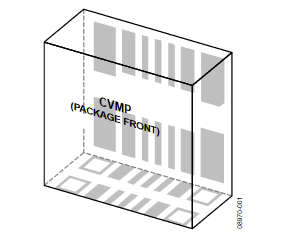
\includegraphics[keepaspectratio, height=.3\textheight, width=\textwidth]{docs/vmp.png}
		\caption{Vertical Mount Package}
		\label{fig:my_label}
	\end{figure}
	
	According to the \href{https://web.archive.org/web/20200818133905/https://www.analog.com/media/en/package-pcb-resources/material-declaration/lcc/LCC_V_14L(ey-14-1).PDF}{material declaration}, the substrate is aluminum-oxide based, a common ceramic solution and the metal lid iron/nickel. The plating is gold/nickel. The ceramic base will have better thermal performance than the rest of the epoxy mold compounds. So for this package a different model approach may be required. But it should be noted that what is referred exactly as lid and base in terms of dimensions is unclear. 
	
	\subsection{LGA}
	
	The Land Grid Array (LGA) is an advanced packing method and this is for the COMMS RFFM6406 UHF TX-RX. It is leadless and it has an exposed thermal pad. Material declaration is missing. We can assume for now that it is plastic based (so we can use LQFP thermal properties as reference), because according to \href{https://web.archive.org/web/20200818134018/https://www.nxp.com/docs/en/application-note/AN2265.pdf}{NXP's application note}, the LGA in the construction is identical with the PBGA except the solder balls. 
	
	About plating: "The LGA pad uses the same 0.1 um to 0.9 um of electroless gold plating over electroless nickel as has been used reliably for many years in the traditional BGA configuration" \cite{nxpplating}.
	
	
	\subsection{Thermal characteristics}
	
	Until now we have investigated the anatomy and the materials of some IC packages along with their properties. Regarding the thermal modeling, in order for the supplier to give to the users an overview of the thermal performance, a standardized approach is usually followed. Under the section "Thermal characteristics" or "Thermal metrics" in datasheets,  there is data that can be used to evaluate the junction temperature. This data is produced by thermal simulations with conditions and test boards suggested by various standards.
	
	The so called \textbf{theta} values are the indicators of this performance and some of them, using the resistor model, are defined as the thermal resistance between 1) die and ambient, 2) die and case, 3) case and ambient.
	
	\begin{figure}[h!]
		\centering
		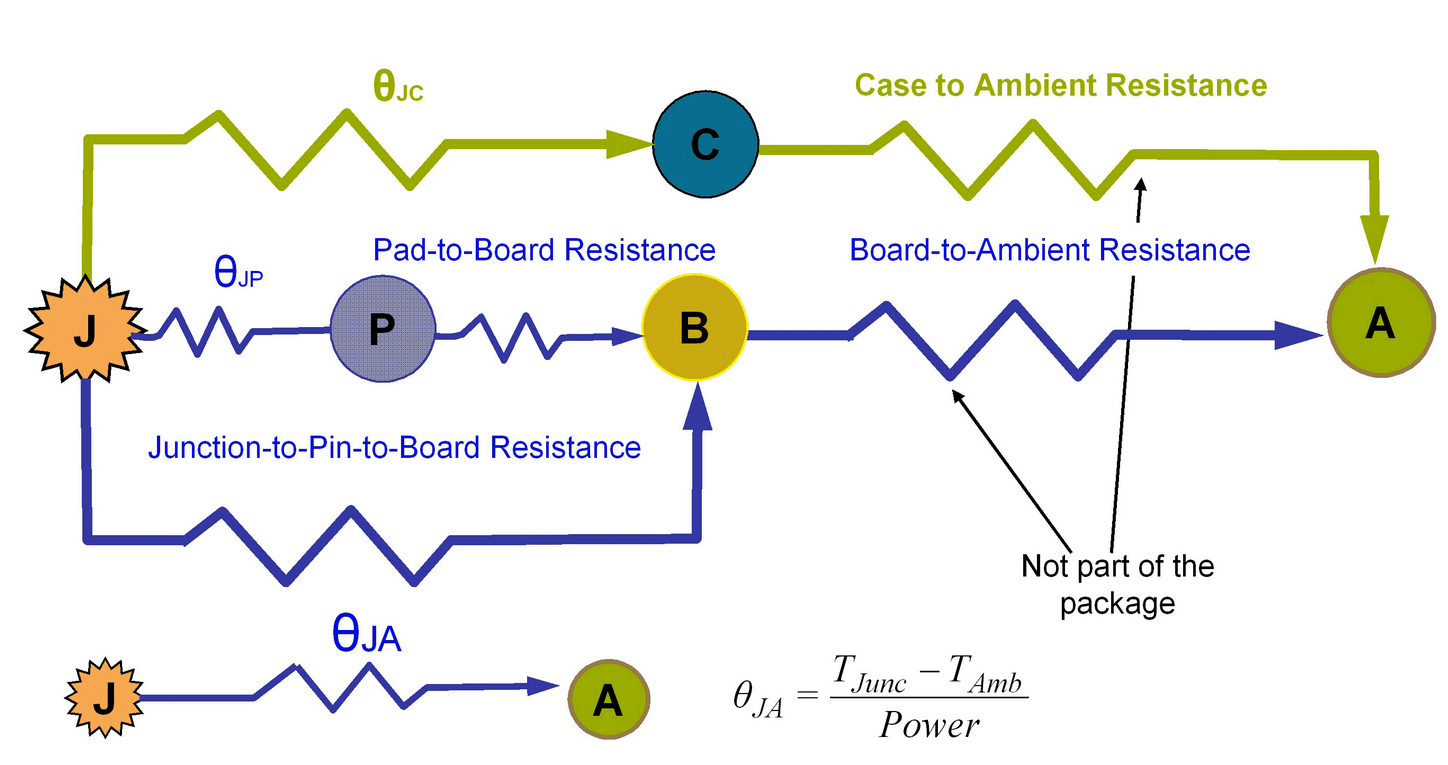
\includegraphics[keepaspectratio, width=\textwidth, height=.25\textheight]{docs/resistor_model.png}
		\caption{A resistor model of an IC package thermal analysis \small{(\href{https://web.archive.org/web/20200818173736/https://www.edn.com/ensuring-the-thermal-integrity-of-your-ic-package-pc-board-design/}{image source})}} 
		\label{fig:my_label}
	\end{figure}
	
	But most of the times, these theta values are not constant and not applicable for every experimental case. According to the \href{https://web.archive.org/web/20200818184640/https://www.st.com/resource/en/application_note/dm00395696-thermal-management-guidelines-for-stm32-applications-stmicroelectronics.pdf}{ST thermal management document}, this data is used for an early assessment and not for a detailed approach. But the questions still remains: Can you use these thermal metrics to your analysis/simulation?
	
	Another usage of this data is to compare the thermal performance of different components. This is only accurate though if all the the values are based on the same standard.
	
	\subsubsection{External links}
	\begin{itemize}
		\item \href{https://web.archive.org/web/20200818132243/https://www.ti.com/lit/an/spra953c/spra953c.pdf}{TI Semiconductor and IC Package Thermal Metrics}
		\item \href{https://web.archive.org/web/20200818123847/https://www.nxp.com/docs/en/white-paper/BasicThermalWP.pdf}{NXP Thermal analysis of semiconductor devices}
	\end{itemize}
	
	
	\section{PCB}
	
	In the "Buildup" section, when ordering from Eurocircuits, there are many options for the thickness of the core FR4 and the copper foils.
	
	Approximate thickness values for a typical 4 layer board 1.55\footnote{In the board thickness only the copper and the dielectric is taken into account} mm:
	\begin{itemize}
		\item FR4:  1,4 mm
		\item Copper:  0,15 mm
		\item Soldermask: 35 - 40 microns
		\item Surface treatment: 20 - 25 microns
		\item Conformal coating: -
	\end{itemize}
	
	
	\begin{figure}[h!]
		\centering
		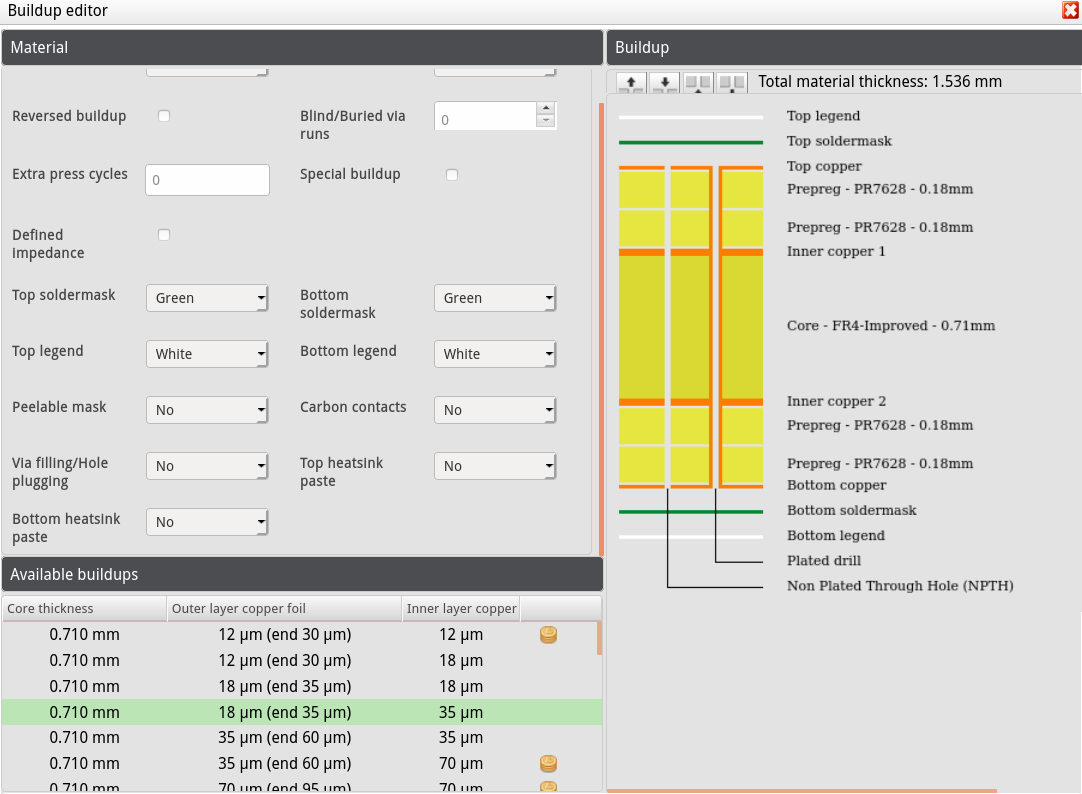
\includegraphics[keepaspectratio, height=0.35\textheight, width=\textwidth]{docs/stackup.png}
		\caption{A typical 4-layer board ordered from Eurocircuits}
		\label{fig:my_label}
	\end{figure}{}
	
	
	\subsection{FR4}
	
	\textbf{IS400}, for example, is one of the  available options by Eurocircuits for FR4 substrate. In general FR4 in contrast with others more expensive ceramic substrates based on aluminum and silicon has a low thermal conductivity. So if there are thermal issues, FR4 replacement is also a choice. Usually ceramic substrate thermal conductivity (typically 10 W/mK) can be 10 or even 100 times greater than FR4 (typically 0,3 W/mK) \cite{zotero-57, zotero-56}. For the IS400 we have:
	
	\subsubsection{Documentation}
	
	\begin{itemize}
		\item \href{https://www.isola-group.com/products/all-printed-circuit-materials/is400/}{All files}
		\item \href{https://web.archive.org/web/20200818140037/https://www.isola-group.com/wp-content/uploads/IS400MaterialDeclaration2007.pdf}{Material declaration}
		\item \href{https://web.archive.org/web/20200818140113/https://www.isola-group.com/wp-content/uploads/data-sheets/is400.pdf?v=1585950502}{Datasheet}
	\end{itemize}
	
	
	\subsubsection{Thermal properties}
	
	\begin{center}
		\tablehead{\hline}
		\tabletail{\hline}
		%\tablecaption{FR4 samples of thermal properties}
		\begin{mpsupertabular}{|c|c|c|}
			\multirow{1} {*} {Thermal conductivity (W/mK)\footnote{Reference for the thermo-optical properties \href{https://web.archive.org/web/20200818140113/https://www.isola-group.com/wp-content/uploads/data-sheets/is400.pdf?v=1585950502}{datasheet}}} & 0,36 \\  
			\hline
			\multirow{1} {*} {Heat capacity (J/kg*K) \footnote{References for the thermo-optical properties Figure \ref{fig:fr4properties}}} & 1000 \\ 
			\hline
			\multirow{1} {*} {Emissivity  \footnote{References for the thermo-optical properties Figure \ref{fig:fr4emiss}}} & 0,9  \\
			\hline
			\multirow{1} {*}{Absorptivity  \footnote{References for the thermo-optical properties Figure \ref{fig:fr4emiss}}} & 0,49 \\
			\hline
		\end{mpsupertabular}
	\end{center}
	
	
	
	
	\textbf{Issue}: The thermal properties emissivity, absorptivity and heat capacity are missing from the datasheet. Alternatively, estimations can be made from other abstract resources (e.g. makeitfrom, wikipedia, handbooks, other applications notes from manufacturers, engineering toolbox).
	\newline
	
	
	\subsection{Copper}
	
	Detailed data about the Eurocircuit's copper foil is missing from their documents. The only information available is the thickness and the overall process of the fabrication. So we could probably assume that the thermal properties will be the same with the well-known pure copper.
	
	
	\begin{center}
		%\tablehead{\hline}
		%\tabletail{\hline}
		\tablecaption{Copper samples of thermal properties}
		\begin{tabular}{|c|c|}
			\hline
			\multirow{2} {*} {Thermal conductivity (W/mK)} & 401 \cite{wiki:copper} \\ & 20 \cite{chandrashekar2017} \\ & 392 \cite{pecht1998electronic} \\
			\hline
			\multirow{1} {*} {Heat capacity (J/kgK)} & 0,385 \cite{wiki:tableheat}\\
			\hline
			\multirow{2} {*} {Emissivity}  & 0,87 oxidized \cite{wiki:emissivity}\\ & 0,8 \cite{chandrashekar2017}\\ & 0,8 coil tape \cite{nasa} \\ & 0,55 foil tape, tarnished \cite{boushon2018} \\ & 0,31 beryllium \cite{boushon2018}\\  & 0,04 polished \cite{wiki:emissivity}\\  & 0,03 electroplated \cite{chandrashekar2017}\\ & 0,3 buffed \cite{boushon2018}\\ 
			\hline
			\multirow{2} {*}{Absorptivity} & 0,04 foil tape, tarnished \cite{boushon2018}\\ & 0,03 buffed \cite{boushon2018} \\ & 0,31 beryllium \cite{boushon2018} \\ 
			\hline
		\end{tabular}
	\end{center}
	
	\section{PC104}
	
	I am going artfully redirect you to the following reference:
	
	"Concerning the conductive links between the PCBs, there are two main heat flow paths: through the spacers and through the connector. According to the PC/104 specification, the connector is made up of 104 phosphor bronze pins and only pins contributes to the link since connector’s housing height is such as there is no contact with the above PCB". Thermal conductivity of Phosphor bronze 75 W/mK \cite[p.104]{jacques2009thermal}. 
	
	
	
	\section{Lessons learned}\label{lessons_learned}
	
	In the beginning of the research, the thinking path about finding materials was oriented to search for each manufacturer the "material declaration" document. Knowing the materials, we will be able to find their thermal properties. But for each part of the component we are interested (e.g. encapsulation), a mixture of materials is used. Thus we assume that we need to focus on the material with the highest concentration. Later for optimization we could find the thermal properties of all of them along with a formula to calculate the overall performance. This approach may be not be valid and probably should be avoided. The primary reason is that this concept is error-prone and adds significant load, trying to demystify the thermal properties of each material and for each component, lacking at the same time the resources to find reliable data. A more abstract way of thinking is may required. So as it is mentioned before, in the IC packaging, a process which several chemical compounds are involved, we can safely assume the general model of an epoxy mold compound for the plastic packages. The same homogenous approach applies for the FR4 too, but fortunately we were able to find experimental data for our case provided by the supplier.
	
	
	
	When approaching the properties of a mixture of materials, there are many chances that what you are looking for has some kind of a code-name, a specific composition. These are common alloys and it would be helpful to identify it by checking the composition from the material doc. 
	
	
	\subsection{Modeling}
	\label{subsec:modeling}
	
	
	In some case we found modeling the PCB as an homogenous material and it is worth mentioning the following:
	
	
	"Printed circuit boards (PCBs) are complex structures usually made up of layers of copper and glass fiber reinforced (fiberglass) epoxy resin, making them difficult to model directly. The layered structure and sharp difference in thermal conductivity between materials leads to highly anisotropic thermal conductivities. Since actually modeling each layer at such small scales and in such detail requires a lot of computational effort and time, the typical practice is to treat the circuit board as a homogenous material and use an effective thermal conductivity" \cite{peake2014cubesat}
	
	\begin{figure}[h!]
		\centering
		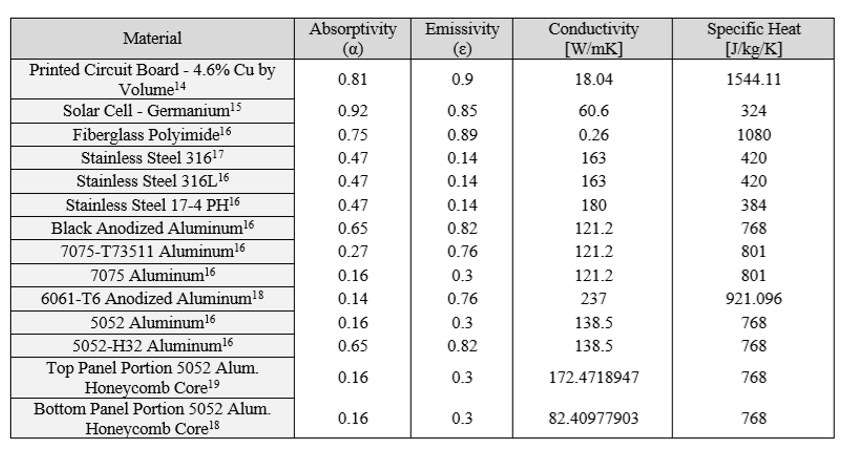
\includegraphics[keepaspectratio, height=0.3\textheight, width=\textwidth]{docs/material_properties_table.png}
		\caption{Material properties table  \cite[p.115]{zotero-47}}
		\label{fig:my_label}
	\end{figure}
	
	A list of concerns:
	
	\begin{itemize}
		\item "An especially intriguing problem shows up when printed circuit boards are part of the analysis. The values for the thermal conductivities of PCB’s cited in literature are mostly conductivities of the epoxy in the direction normal to the PCB. However, these values are useless in practice because: a) the thermal conductivity of the reinforced epoxy can be highly anisotropic, b) the in-plane thermal conductivity is much more important from a practical point of view, c) the very complex patterns of metal tracks and layers will considerably influence the thermal conduction behavior" \cite{lasance2002}
		\item ”Regarding the material properties it was found that small changes, e.g.  adding a layer of copper to the circuit board, can significantly decrease the resulting temperatures.  This is due to the improved in-plane conductivity, as copper has an unequally higher conductivity than FR4(Cu=394W/mK compared to FR4=0.3W/mK).” \cite{reiss2012} 
		\item "While the temperature changes significantly, the overall pattern of the heat distribution remains relatively unchanged. The largest change is the difference between the highest and lowest temperatures, which grows from 6 K to 52 K between $\epsilon$ = 0.02 and $\epsilon$ = 0.82. Overall, it is clear that emissivity plays a very significant role in the spacecraft temperature. This was expected, since radiation as a mode of heat transfer is far more important in the near vacuum of space, and is the only mode by which heat can be transferred away from the satellite." \cite{peake2014cubesat}
		\item "Because a satellite in orbit is surrounded by the vacuum of space, its only
		thermal interaction with its environment is through radiation" \cite{vanoutryve2008}.
		
		"The aluminum external surface is the only \textbf{external} part which can be used to control the temperature by modifying the optical properties of the material (with an adequate surface treatment); indeed, the optical properties of the solar cells and of the PCB that are mounted to them cannot be modified" \cite{paris2015}.
		
		Also in the TIGRIsat's simulations , when they didn't take into account the surface treatment of the aluminum structure/rails, the temperature had exceed the maximum one. The reason behind this was the big difference between aluminum's absorptivity (0,379) and emissivity (0,08) due to the aforementioned assumption that there wasn't any surface treatment \cite{paris2015}. Based on that, the input data of "critical" components should be investigated thoroughly and changing the thermal-optical properties can be also part of the strategy.
	\end{itemize}
	
	
	\subsection{Uncertainty and thermal properties}
	
	
	Many thermal properties can be indexed. This is true. But most of the times, conflicts will emerge. There is a variety of values referred to the same material and thermal data as an input is also a part of the engineering process. Assumptions and estimations are a common thing to do and they are function of the general modeling approach. Do I need this property, can I model it with another way, how uncertain is this thermal data, is this material oxidized or even if it isn't can I benefit assuming that it is? 
	
	\begin{itemize}
		\item "... models of the electrical and electronic components has been created, despite the \textbf{difficulty} of determining their thermal and optical properties." 
		
		"Indeed, the \textbf{actual} structure of TIGRIsat is anodized but the actual value of $\alpha$  and $\epsilon$ are \textbf{unknown}" \cite{paris2015}
		
		\item "Often information for properties of individual material is \textbf{unavailable} and, where possible, in-house testing using an emissometer should be performed to acquire it." \cite{mccarron2018developing}
		
		
		\item "However, there may be quite a few uncertain or inaccurate input parameters existing in the thermal mathematical model (TTM), which may affect the analysis accuracy, including thermal contact resistance between contacting parts, unit thermal properties (such as thermal capacitance, thermal conductivity, infrared emissivity, and solar absorptivity), unit power dissipation, etc. Therefore, a thermal balance test is essential to verify the basic thermal design and to assure that the TMM is reliable for the temperature prediction because the input parameters are proved to be valid" \cite{tsai2004overview}
		
		
		
		
		\item About the accuracy of experimental and numerical thermal analysis of electronic systems: "The final conclusion is inevitable: the situation when all computations at the system level can be used for accurate temperature prediction is still a long way off" \cite{lasance2002}
	\end{itemize}
	
	With all of that being said we can understand that we can't trust the thermal data. Experimental data for each application along with tests is a necessary part of the design-cycle. In prototypes, thermocouples and infrared cameras can be used in the same way that oscilloscopes are being used for the electrical domain.
	
	\section{Databases}\label{Databases}
	
	\begin{itemize}
		\item Glenn R Blackwell.The electronic packaging handbook.  CRC Press, 2017
		\item Safa Kasap and Peter Capper.Springer handbook of electronic and photonic materials.Springer, 2017
		\item Rao R Tummala et al.  Fundamentals of microsystems packaging.  2001
		\item R.P.  Chhabra.CRC Handbook of Thermal Engineering.   Mechanical  and  AerospaceEngineering Series. CRC Press
		\item  M. Pecht, R. Agarwal, F.P. McCluskey, T.J. Dishongh, S. Javadpour, and R. Mahajan.Electronic Packaging Materials and Their Properties.  Electronic Packaging. Taylor Francis
		\item D.G. Gilmore and M. Donabedian.Spacecraft Thermal Control Handbook: FundamentalTechnologies.  Spacecraft Thermal Control Handbook. Aerospace Press
		\item https://theengineeringmindset.com/specific-heat-capacity-of-materials/
		\item \href{https://www.makeitfrom.com/}{makeitfrom.com}. A general online database for various materials. Mined from Wikipedia references
		\item \href{https://www.engineeringtoolbox.com/}{The Engineering Toolbox}. This reference is used quite a lot.
		\item \href{https://web.archive.org/web/20200818140417/https://monarchserver.com/Files/pdf/TableofEmissivity.pdf?14860239451575071105}{Table of Total Emissivity}
		\item \href{https://web.archive.org/web/20200818140448/http://www.solarmirror.com/fom/fom-serve/cache/43.html}{Table of absorptivity and emissivity of common materials and coatings}
		\item \href{https://drive.google.com/file/d/1nZOXnBw6FdrzXW1Nm0Q7n0jfy6kBI26J/view?usp=sharing}{Thermal Properties of Plastic Materials}
		\item \href{https://web.archive.org/web/20200818140510/http://www.infrared-thermography.com/material.htm}{Emissivity Values for Common Materials}
		\item \href{https://cindasdata.com/Applications/MPMDDEMO}{CINDAS LLC}. This is an interesting database. There are thermal properties even for very specific mold compounds types like "Sumitomo EME-6300HS" (just to remind you, ST is using Sumitomo type mold compounds as encapsulation) but it is proprietary.
	\end{itemize}
	
	
	\section{List of tables}\label{list_tables}
	
	
	
	\begin{figure}[h!]
		\centering
		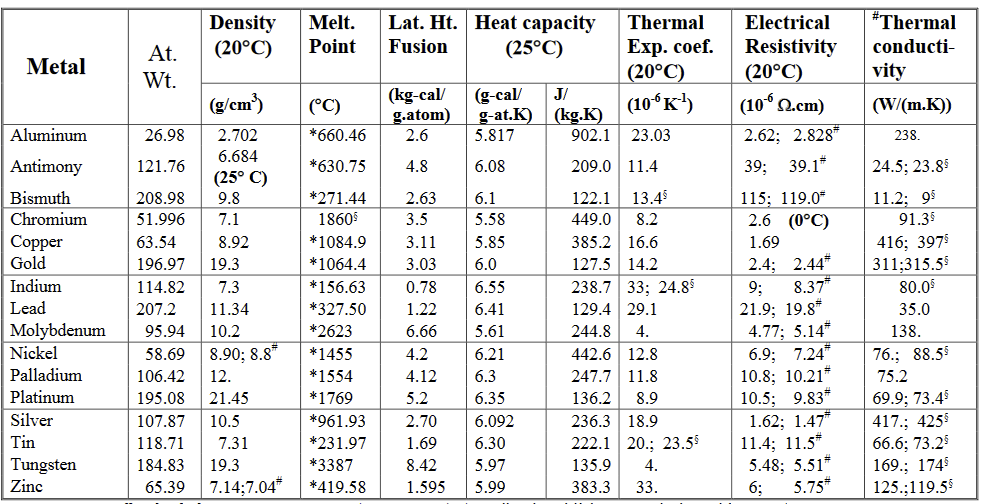
\includegraphics[width=\linewidth]{docs/mist_heat_capacity.png}
		\caption{\cite[p.37]{solder}}
		\label{fig:metal_table_1}
	\end{figure}
	
	\begin{figure}[h!]
		\centering
		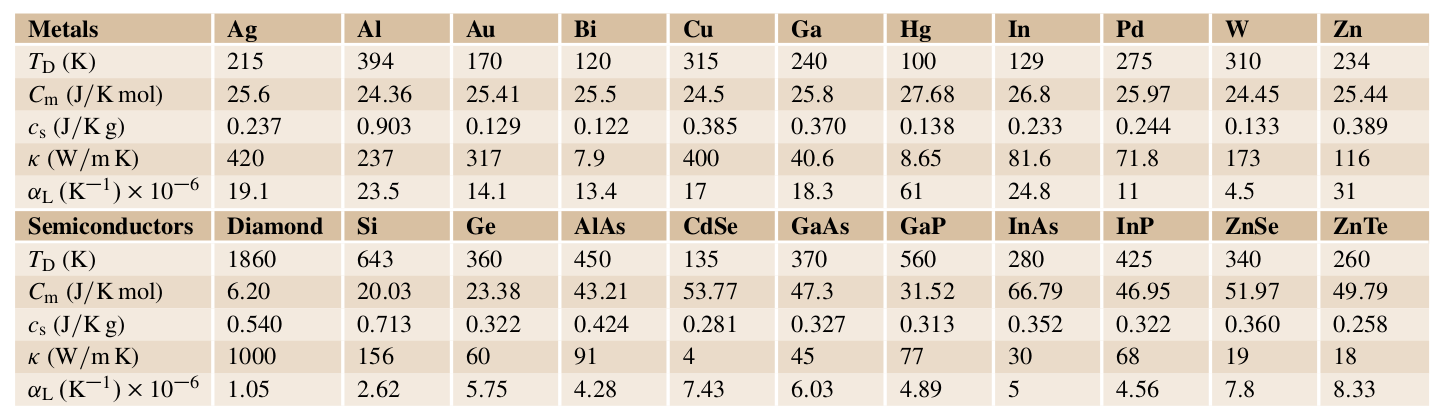
\includegraphics[width=\linewidth]{docs/table_properties_springer.png}
		\caption{\cite[p.428]{kasap2017springer}}
		\label{fig:metal_table_2}
	\end{figure}
	
	\begin{figure}[h!]
		\centering
		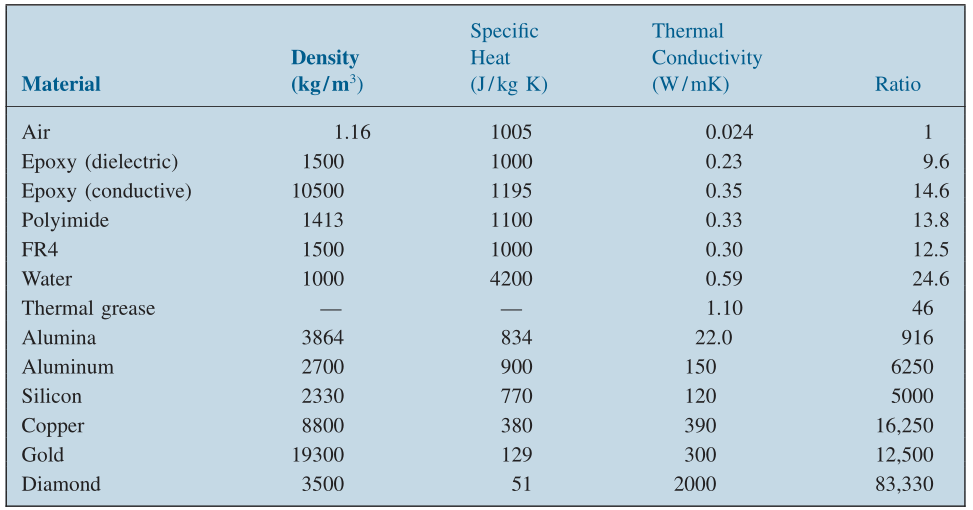
\includegraphics[width=\linewidth]{docs/table_properties_bible.png}
		\caption{\cite[p.222]{tummala2001fundamentals}}
		\label{fig:fr4properties}
	\end{figure}
	
	\begin{figure}[h!]
		\centering
		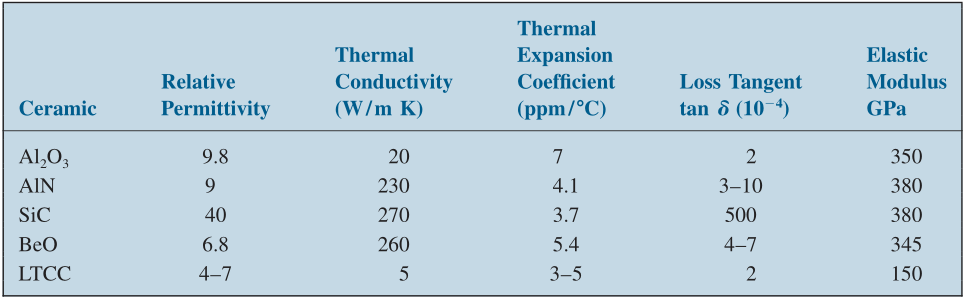
\includegraphics[width=\linewidth]{docs/table_ceramics_bible.png}
		\caption{\cite[p.718]{tummala2001fundamentals}}
		\label{fig:my_label}
	\end{figure}
	
	
	
	\begin{figure}[h!]
		\centering
		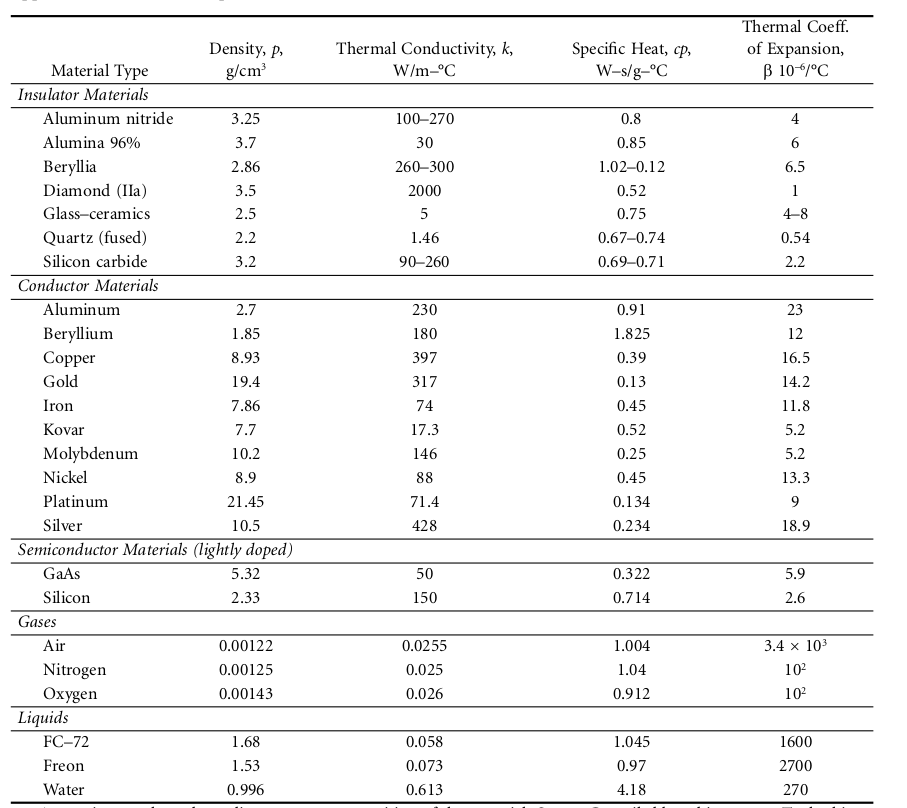
\includegraphics[width=\linewidth]{docs/table_properties_blackwell_handbook.png}
		\caption{\cite[p.408]{blackwell2017electronic}}
		\label{fig:springer_properties}
	\end{figure}
	
	\begin{figure}[h!]
		\centering
		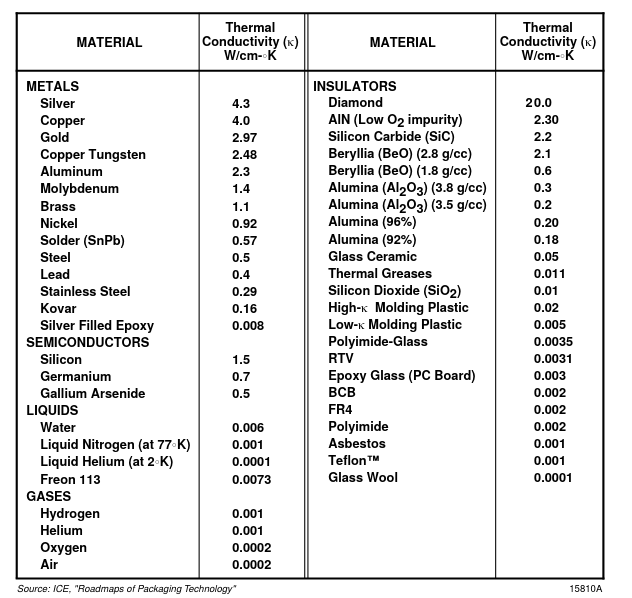
\includegraphics[width=\linewidth]{docs/table_properties_smith.png}
		\caption{\cite[6-14]{chip}}
		\label{fig:intel_conduct}
	\end{figure}
	
	\begin{figure}[h!]
		\centering
		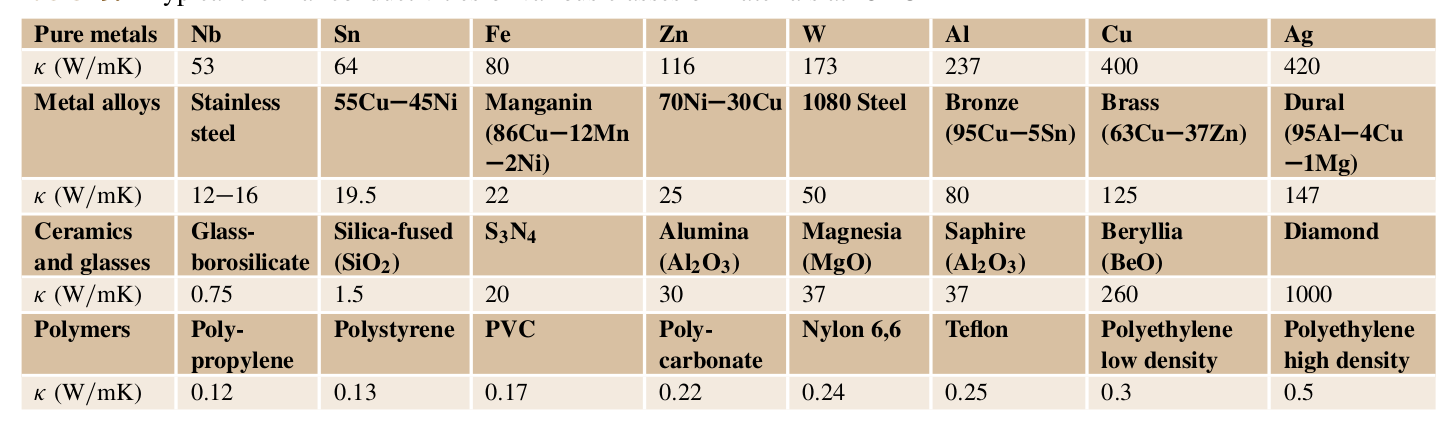
\includegraphics[width=\linewidth]{docs/table_properties_springer2.png}
		\caption{\cite[p.431]{kasap2017springer}}
		\label{fig:my_label}
	\end{figure}
	
	\begin{figure}[h!]
		\centering
		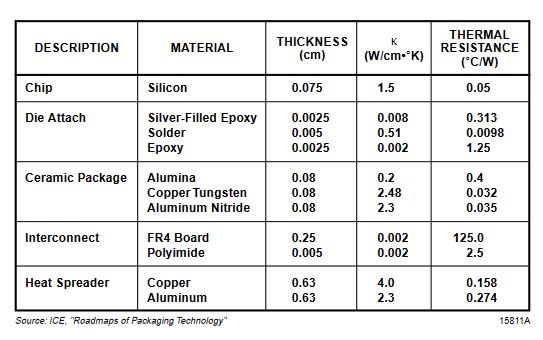
\includegraphics{docs/chip_properties.png}
		\caption{\cite[p.6-12]{chip}}
		\label{fig:my_label}
	\end{figure}
	
	\begin{figure}[h!]
		\centering
		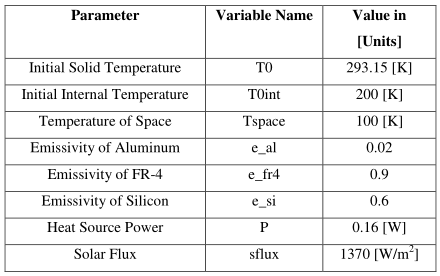
\includegraphics[keepaspectratio, width=\textwidth]{docs/emissivity_silicon_fr4.png}
		\caption{\cite[p.41]{peake2014cubesat}}
		\label{fig:my_label}
	\end{figure}
	
	
	\begin{figure}[h!]
		\centering
		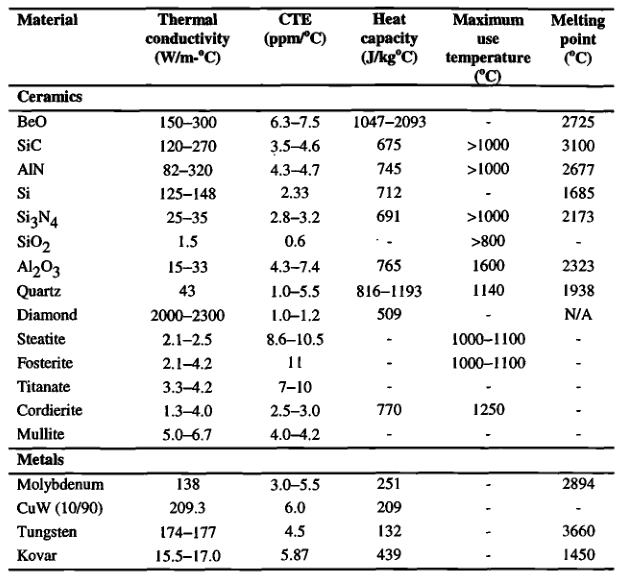
\includegraphics[keepaspectratio, width=\textwidth]{docs/substrates.png}
		\caption{Substrates \cite[p.32]{pecht1998electronic}}
		\label{fig:my_label}
	\end{figure}
	
	\begin{figure}[h!]
		\centering
		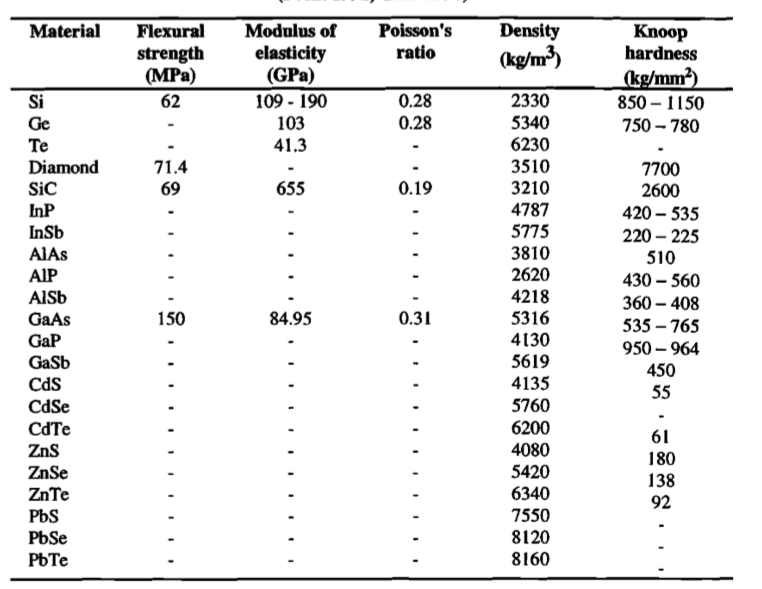
\includegraphics[keepaspectratio, width=\textwidth]{docs/density_table.png}
		\caption{\cite[p.24]{pecht1998electronic}}
		\label{fig:my_label}
	\end{figure}
	
	\begin{figure}[h!]
		\centering
		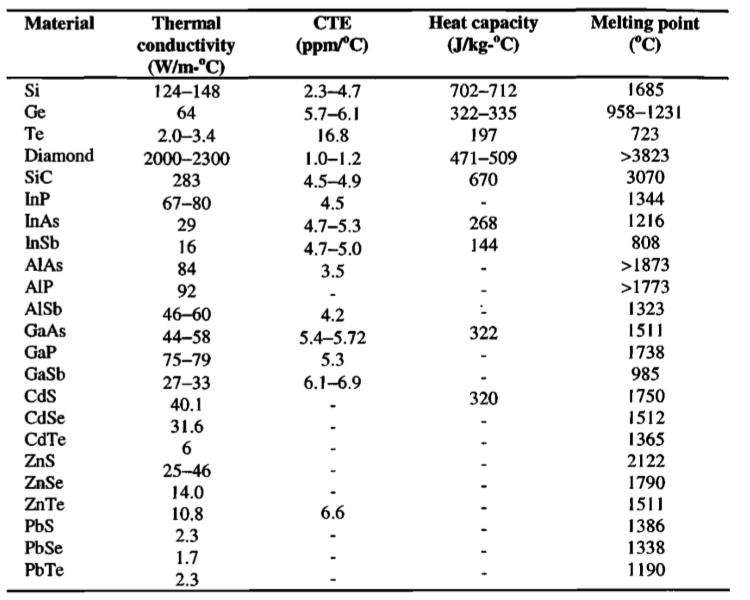
\includegraphics[keepaspectratio, width=\textwidth]{docs/material_overall_properties.png}
		\caption{\cite[p.25]{pecht1998electronic}}
		\label{fig:my_label}
	\end{figure}
	
	\begin{figure}[h!]
		\centering
		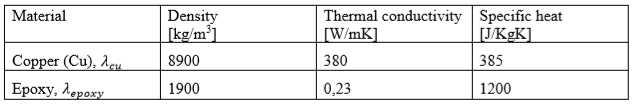
\includegraphics{THE/AcubeSAT-THE-BH-032/docs/homo_pcb.png}
		\caption{\cite[p.20]{airborne}}
		\label{fig:my_label}
	\end{figure}
	
	
	\begin{figure}[h!]
		\centering
		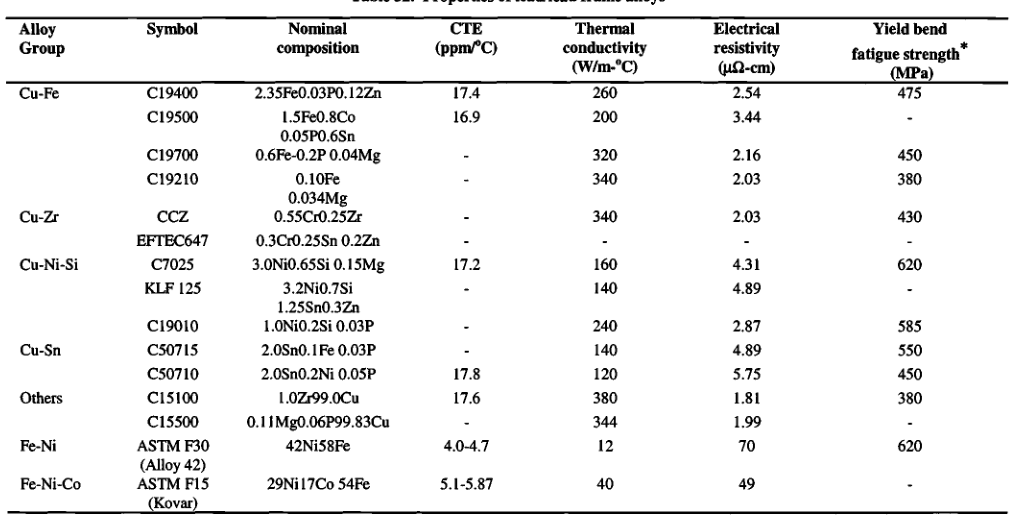
\includegraphics[keepaspectratio, width=\textwidth]{docs/copper_alloys_blackwell.png}
		\caption{\cite[p.55]{pecht1998electronic}}
		\label{fig:copper_alloys}
	\end{figure}
	
	\begin{figure}[h!]
		\centering
		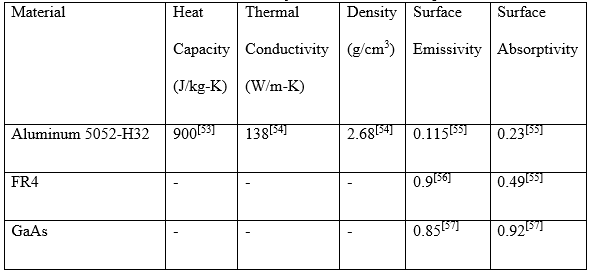
\includegraphics[keepaspectratio, width=\textwidth]{docs/fr4_emiss.png}
		\caption{\cite[p.93]{rathbun2017design}}
		\label{fig:fr4}
	\end{figure}
	
	\begin{figure}[h!]
		\centering
		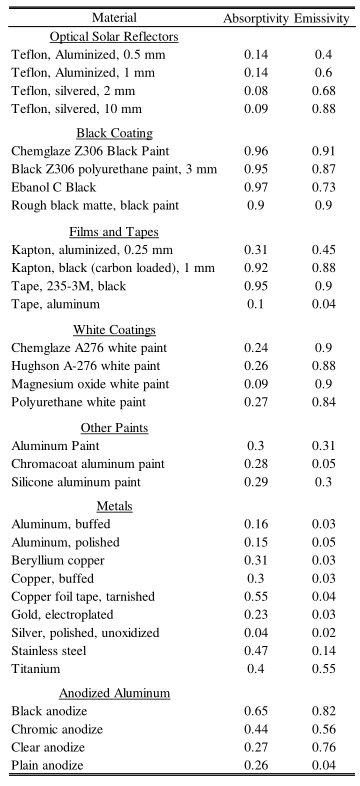
\includegraphics[keepaspectratio, height=.8\textheight, width=\textwidth]{docs/small_sat_properties.png}
		\caption{\cite[p.111]{boushon2018}}
		\label{fig:fr4emiss}
	\end{figure}
	
	\begin{figure}[h!]
		\centering
		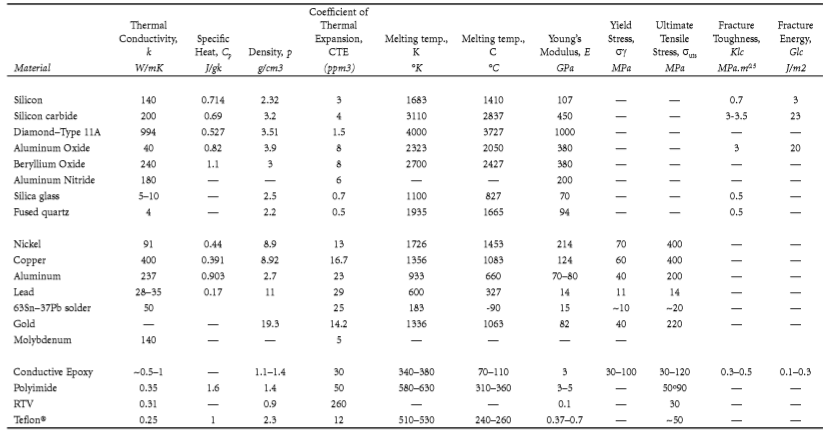
\includegraphics[keepaspectratio, height=.8\textheight, width=\textwidth]{docs/blackwell_prope.png}
		\caption{Metals \cite[p.526]{blackwell2017electronic}}
		\label{fig:emissivity_table}
	\end{figure}
	
	\begin{figure}[h!]
		\centering
		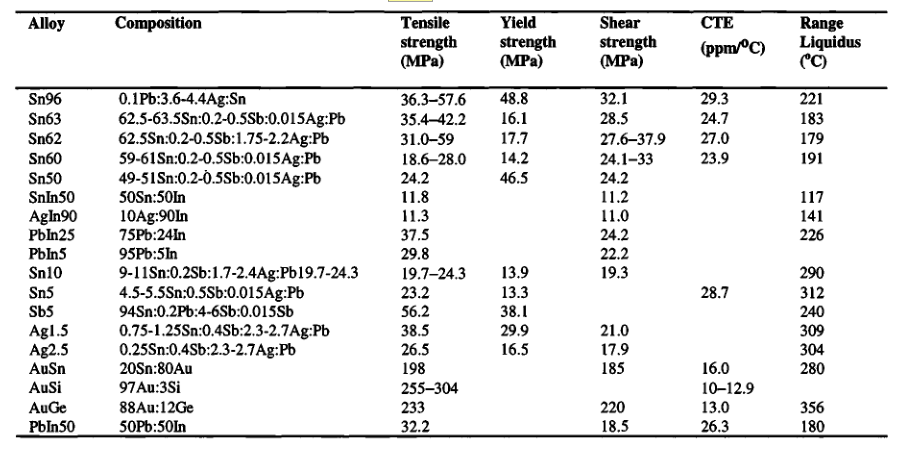
\includegraphics[keepaspectratio, height=.8\textheight, width=\textwidth]{docs/soldes.png}
		\caption{Solders, \cite[p.53]{pecht1998electronic}}
		\label{fig:metals}
	\end{figure}
	
	\begin{figure}[h!]
		\centering
		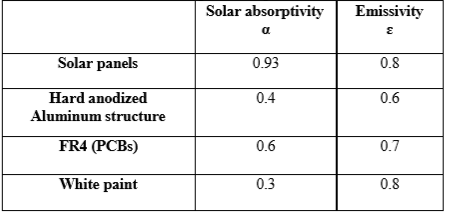
\includegraphics[keepaspectratio, height=.4\textheight, width=\textwidth]{THE/AcubeSAT-THE-BH-032/docs/thermoptic_fr4.png}
		\caption{\cite{ganti2017design}}
		\label{fig:thermoopticfr4}
	\end{figure}
	
	\begin{figure}[h!]
		\centering
		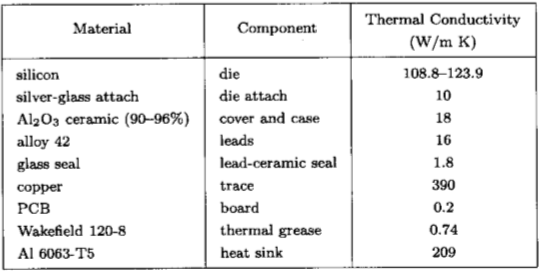
\includegraphics[keepaspectratio, height=.4\textheight, width=\textwidth]{THE/AcubeSAT-THE-BH-032/docs/pcb_properties.png}
		\caption{\cite{teng1997thermal}}
		\label{fig:pcb_level}
	\end{figure}
	
	\begin{figure}[h!]
		\centering
		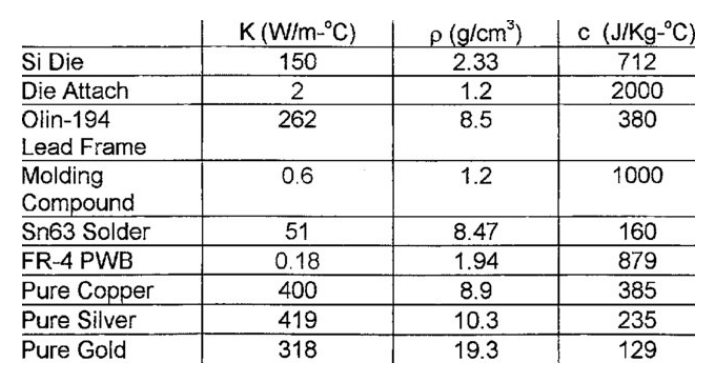
\includegraphics[keepaspectratio, height=.25\textheight, width=\textwidth]{docs/package_properties_no1.png}
		\caption{\cite{kuo1998ic}}
		\label{fig:tab_1}
	\end{figure}
	
	\begin{figure}[h!]
		\centering
		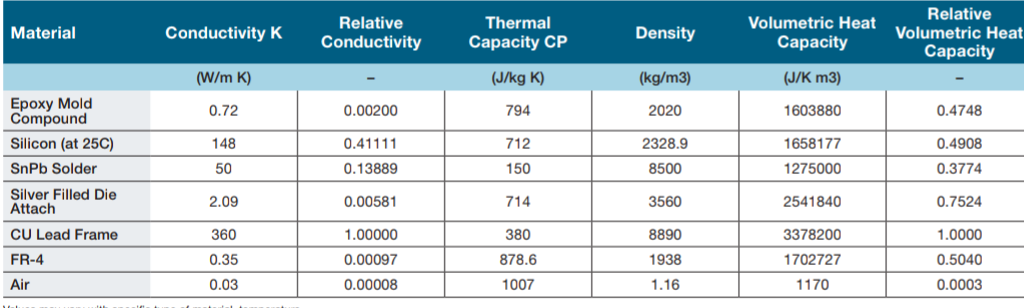
\includegraphics[keepaspectratio, height=.25\textheight, width=\textwidth]{docs/package_properties_no2.png}
		\caption{\cite{nxp:material}}
		\label{fig:tab_2}
	\end{figure}
	
	\begin{figure}[h!]
		\centering
		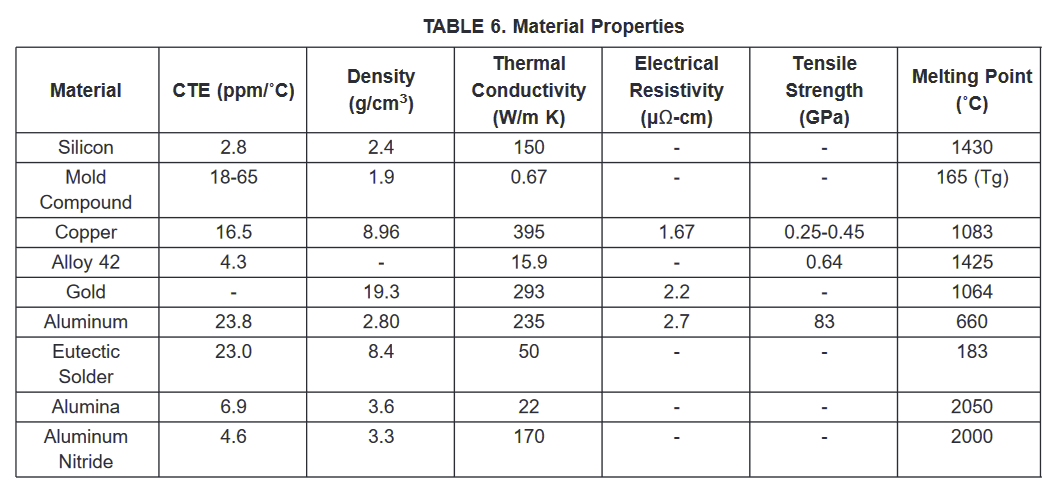
\includegraphics[keepaspectratio, height=.25\textheight, width=\textwidth]{docs/TI_ic_assembly.png}
		\caption{\cite{ti:material}}
		\label{fig:tab_3}
	\end{figure}
	
	\begin{figure}[h!]
		\centering
		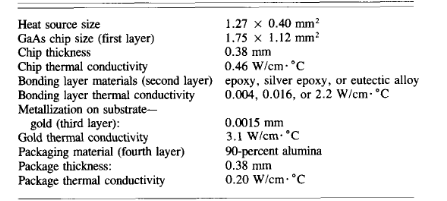
\includegraphics[keepaspectratio, height=.25\textheight, width=\textwidth]{docs/package_properties_no3.png}
		\caption{\cite{49036}}
		\label{fig:tab_4}
	\end{figure}
	
	\begin{figure}[h!]
		\centering
		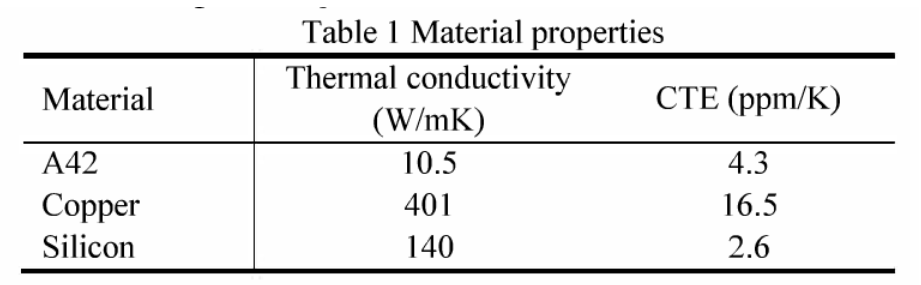
\includegraphics[keepaspectratio, height=.15\textheight, width=\textwidth]{docs/copper_plating_thickness.png}
		\caption{\cite{Li2012EffectsOC}}
		\label{}
	\end{figure}
	
	\clearpage
	
	\bibliographystyle{plain}
	\bibliography{thermal.bib}
	
\end{document}
